\chapter{Experimental Results}
\pagestyle{fancy}\lhead{\textbf \footnotesize\it{Experimental Results}}
\pagestyle{fancy}\chead{} \pagestyle{fancy}\rhead{}
\pagestyle{fancy}\lfoot{\textbf {\small\it{Univ-Mascara/Computer Science: 2025}}} 
\pagestyle{fancy}\cfoot{} \pagestyle{fancy}\rfoot{\thepage}
%%%%%%%%%%%%%%%%%%%%%%%%%%%%%%%%%%%%%%%%
\section{Introduction}\label{start6}
In this chapter, we present the experimental results of applying our novel algorithm to SASRec and compare its performance with SASRec tested using MOL. The goal of these experiments is to assess the effectiveness of our approach in improving recommendation accuracy, model efficiency, and overall performance metrics.

\section{Recommendation System Overview}
Modern technology and online services have enabled unprecedented access to vast amounts of data. However, this abundance of information creates an overload, making it harder for users to find relevant content efficiently. Recommender systems address this by filtering information and delivering personalized suggestions, saving users time and effortz\cite{Roy2022}. These systems are now integral to platforms like e-commerce, television programs\cite{5174476}, e-learning\cite{WANG201110831}, tourism, and more, though further improvements are needed to enhance their versatility and accuracy.
\begin{figure}[ht]
	\centering
	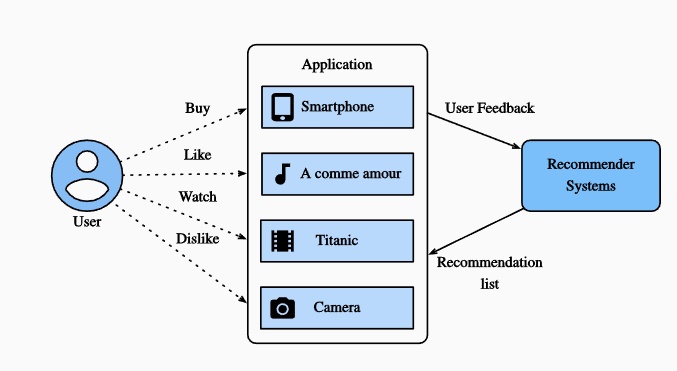
\includegraphics[width=0.5\linewidth]{Figures/RS.png}
	\caption{Recommendation System Process\cite{zhang2021recsys}}
	\label{Recommendation_System _Process}	
\end{figure}
\subsection{SASRec: Self-Attentive Sequential Recommendation}
Sequential recommendation systems aim to predict a user’s next interaction based on their historical behavior while incorporating contextual information from recent actions. However, effectively capturing patterns in sequential data is challenging due to the exponential growth of the input space as more past interactions are considered.\cite{kang2018selfat}
\subsection{SASRec Model Architecture}
SASRec leverages self-attention to assign adaptive weights to past items at each time step. The key components include:\\
\textbf{ Embedding Layer:} Converts user interactions into dense vector representations. \\
\textbf{ Self-Attention Layer: }Captures dependencies between different interactions in the sequence, allowing for long-range modeling.\\
\textbf{ Point-Wise Feed Forward Network (FFN)}: Enhances feature extraction for better predictions.\\
\textbf{Prediction Layer:} Computes the likelihood of the next interaction based on learned patterns.\\
A visual representation of SASRec’s training process (Figure \ref{the_training_process_of_SASRec}) illustrates how the model uses self-attention to focus on relevant past interactions when making predictions
\begin{figure}[ht]
	\centering
	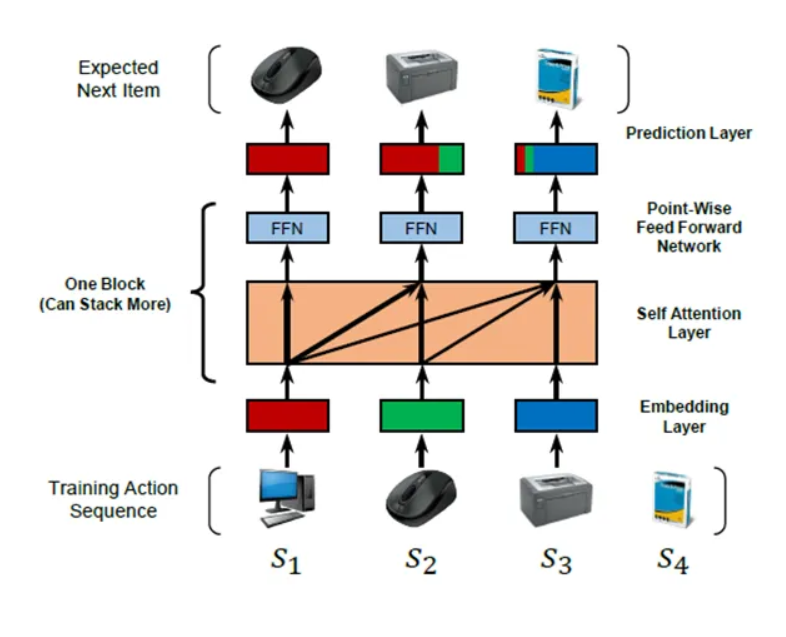
\includegraphics[width=0.6\linewidth]{Figures/sasrec.png}
	\caption{the training process of SASRec\cite{kang2018selfat}}
	\label{the_training_process_of_SASRec}	
\end{figure}
\section{ Datasets}
To evaluate the effectiveness of our proposed algorithm, we conduct experiments on widely used benchmark datasets: MovieLens-100K and MovieLens-1M \cite{Harper2015}. These datasets provide user-item interaction histories, making them well-suited for sequential recommendation tasks. By testing on both a small-scale and a larger dataset, we analyze the model’s performance across different data sparsity levels and user engagement patterns.
\subsection{MovieLens-100K}
MovieLens data sets were collected by the GroupLens Research Project
at the University of Minnesota.This data set consists of:\\
* 100,000 ratings (1-5) from 943 users on 1682 movies. \\
* Each user has rated at least 20 movies. \\
* Simple demographic info for the users (age, gender, occupation, zip)
\subsection{MovieLens-1M}
* 1,000,209 ratings from 6,040 users on approximately 3,900 movies \\
* Data collected from users who joined MovieLens in 2000 \\
* Represents a larger-scale recommendation scenario \\
\section{Experimental Setup}
For both datasets, We utilize the SASRec architecture as our sequential user encoder, a model renowned for achieving state-of-the-art performance in next-item prediction tasks. This architecture processes the user's historical interaction sequence, generating embeddings that encapsulate the user's preferences at each time step. These embeddings serve as the foundation for predicting the next item in the sequence.

The query q represents the user's state at a specific time step, derived from their interaction history. In the MoL (Mixture of Logits) framework, q is transformed into Pq
embeddings through a multi-layer perceptron (MLP). While our hybrid algorithm does not explicitly employ an MLP for this transformation
\subsection{Hyperparameter Settings}
For fair comparison, we maintained consistent architectural choices and training conditions across all experiments , We conducted an extensive hyperparameter analysis comparing both approaches (Hybrid+SAS and MoL+SAS) across different architectural configurations.All experiments were Implemented in TensorFlow and trained on a Google Colab environment with a T4 GPU. We use the Adam optimizer with a learning rate of 0.001. For the hybrid algorithm, we initialize the threshold (Tinit) to 0.3 and adaptively adjust it during training.We discuss detailed hyperparameter settings in table \ref{tab:100k_movies} ,table \ref{tab:1m_movies}

\setlength{\tabcolsep}{1pt} % Increase column padding

\begin{table}[ht]
	\centering
	\large
	\renewcommand{\arraystretch}{1.5} % Increase row spacing
	\resizebox{\textwidth}{!}{  % Scale table to fit width
		\begin{tabular}{|l|c|c|c|c|c|c|c|c|}
			\hline
			\textbf{Model} & \textbf{Max Sequence Length} & \textbf{Embedding Dimension} & \textbf{Number of Heads} & \textbf{Feedforward Dimension} & \textbf{Batch Size} & \textbf{Epochs} & \textbf{Val Loss} & \textbf{Val Accuracy} \\ 
			\hline
			Hybrid+SAS & 50  & 128  & 2 & 128  & 128 & 12 & 5.3036 & 0.1584  \\ \hline
			MoL+SAS    & 50  & 128  & 2 & 128  & 128 & 12 & 5.3152 & 0.1582  \\ \hline
			Hybrid+SAS & 128 & 256  & 4 & 256  & 128 & 10 & 3.6364 & 0.4301  \\ \hline
			MoL+SAS    & 128 & 256  & 4 & 256  & 128 & 10 & 3.6374 & 0.4299 \\\hline
			Hybrid+SAS & 512 & 512  & 4 & 512  & 128 & 10 & 1.2808 & 0.8120 \\ \hline
			MoL+SAS    & 512 & 512  & 4 & 512  & 128 & 10 & 1.3050 & 0.8016 \\\hline
		\end{tabular}
	}
	\caption{Results on 100kMovies dataset}
	\label{tab:100k_movies}
\end{table}


\setlength{\tabcolsep}{1pt} % Increase column padding

\begin{table}[ht]
	\centering
	\large
	\renewcommand{\arraystretch}{1.5} % Increase row spacing
	\resizebox{\textwidth}{!}{  % Scale table to fit width
		\begin{tabular}{|l|c|c|c|c|c|c|c|c|}
			\hline
			\textbf{Model} & \textbf{Max Sequence Length} & \textbf{Embedding Dimension} & \textbf{Number of Heads} & \textbf{Feedforward Dimension} & \textbf{Batch Size} & \textbf{Epochs} & \textbf{Val Loss} & \textbf{Val Accuracy} \\ 
			\hline
			Hybrid+SAS & 50  & 128  & 2 & 128  & 128 & 10 & 4.5721 & 0.1530  \\ \hline
			MoL+SAS    & 50  & 128  & 2 & 128  & 128 & 10 & 4.5733 & 0.1526  \\ \hline
			Hybrid+SAS & 128 & 256  & 4 & 256  & 128 & 10 & 3.4152 & 0.3680  \\ \hline
			MoL+SAS    & 128 & 256  & 4 & 256  & 128 & 10 & 3.4671 & 0.3627  \\ \hline
			Hybrid+SAS & 512 & 512  & 4 & 512  & 128 & 10 & 1.0275 & 0.8350  \\ \hline
			MoL+SAS    & 512 & 512  & 4 & 512  & 128 & 10 & 1.0350 & 0.8276  \\ \hline
			
		\end{tabular}
	}
	\caption{Results on 1M Movies dataset}
	\label{tab:1m_movies}
\end{table}
\subsection{ Impact of Hyperparameters}
Both approaches demonstrate significant performance improvements as model capacity increases, with larger configurations consistently delivering better results. For instance, when increasing the model's capacity such as expanding the (Max Sequence Length: 512, Embedding Dimension: 512, Number of Heads: 4, Feed-Forward Dimension: 512) the hybrid algorithm combined with SASRec (Hybrid+SAS) achieves notable gains, particularly in the most resource-intensive setup. On the ML-100K dataset, Hybrid+SAS reaches a score of\textbf{ 0.8120} compared to the baseline's \textbf{0.8016}, while on ML-1M, it achieves \textbf{0.8350} versus \textbf{0.8276.} The ML-1M dataset generally benefits more from increased capacity, with the performance gap between datasets narrowing as the model scales. While smaller configurations provide a balance of efficiency and performance, the largest configuration, despite its higher computational demands, yields the best results, making it suitable for scenarios where resources are not a constraint. Both approaches show similar benefits from scaling, but Hybrid+SAS maintains a consistent edge in performance.
\section{Evaluation Metrics}
We employ standard ranking metrics widely used in sequential recommendation:

\begin{itemize}
	\item \textbf{Hit Rate at \( k \) (HR@\( k \))}: Measures the proportion of cases where the target item appears in the top-\( k \) recommendations. The HR@\( k \) is computed as:\cite{Tamm_2021}
	\begin{equation}
		\text{HR@}k = \frac{1}{|U|} \sum_{u=1}^{|U|} \mathbb{I}(\text{rank}_u \leq k),
	\end{equation}
	where \( |U| \) is the number of users, \( \text{rank}_u \) is the rank of the target item for user \( u \), and \( \mathbb{I}(\cdot) \) is the indicator function that returns 1 if the condition is true and 0 otherwise.
	
	\item \textbf{Mean Reciprocal Rank (MRR)}:is a ranking quality metric that measures how quickly a system retrieves the first relevant item. It is calculated as the average of reciprocal ranks across all users or queries,MRR ranges from 0 to 1, with higher values indicating better performance \cite{eviden2025mrr}.
	\begin{equation}
		\text{MRR} = \frac{1}{|U|} \sum_{u=1}^{|U|} \frac{1}{\text{rank}_u},
	\end{equation}
	where \( \text{rank}_u \) is the position of the first relevant item for user \( u \) within the top-K results. \\ 
	U represents the total number of users (for recommendation systems) or queries (for information retrieval tasks) in the dataset.
	
	\item \textbf{Normalized Discounted Cumulative Gain (NDCG)}: Assesses the ranking quality while accounting for position importance. The NDCG@\( k \) is computed as:\cite{Tamm_2021}
	\begin{equation}
		\text{NDCG@}k = \frac{1}{|U|} \sum_{u=1}^{|U|} \frac{\text{DCG@}k}{\text{IDCG@}k},
	\end{equation}
	where \( \text{DCG@}k \) is the Discounted Cumulative Gain at position \( k \):
	\begin{equation}
		\text{DCG@}k = \sum_{i=1}^{k} \frac{2^{\text{rel}_i} - 1}{\log_2(i + 1)},
	\end{equation}
	and \( \text{IDCG@}k \) is the Ideal DCG@\( k \), computed by sorting the items by their true relevance scores.
\end{itemize}  
Table \ref{tab:results_tab} summarizes the performance of our hybrid algorithm compared to the MoL-based approach on the MovieLens 100K and 1M datasets, both tested using a Max Sequence Length of 50, an Embedding Dimension of 128, 2 Attention Heads, a Feedforward Dimension of 128, a Batch Size of 128, and trained for 10 epochs 
\section{Results and Analysis}
\begin{table}[h]
	\centering
	\large
	\renewcommand{\arraystretch}{1.3}
	\begin{tabular}{|l|c|c|c|c|c|c|}
		\hline
		\textbf{Model} & \textbf{HR@1} & \textbf{HR@10} & \textbf{HR@50} & \textbf{HR@200} & \textbf{MRR} & \textbf{NDCG} \\ \hline
		\multicolumn{7}{|c|}{\textbf{MovieLens 100K}} \\ \hline
		SASRec+Hybrid & 0.0070 & 0.0775 & 0.2606 & 0.5704 & 0.0363 & 0.1241 \\ \hline
		SASRec+MoL    & 0.0000 & 0.0775 & 0.2887 & 0.5775 & 0.0285 & 0.1182 \\ \hline
		\multicolumn{7}{|c|}{\textbf{MovieLens 1M}} \\ \hline
		SASRec+Hybrid & 0.0464 & 0.1810 & 0.3819 & 0.6159 & 0.0925 & 0.1829 \\ \hline
		SASRec+MoL    & 0.0508 & 0.1799 & 0.3896 & 0.6126 & 0.0971 & 0.1859 \\ \hline
	\end{tabular}
	\caption{Performance Comparison of SASRec+Hybrid and SASRec+MoL on MovieLens 100K and 1M Datasets}
	\label{tab:results_tab}
\end{table}
\subsection{Discussion}
On the ML-100K dataset, our approach shows comparable performance to MoL in terms of \textbf{HR@10 (0.0775 for both)} while achieving better results in\textbf{ MRR (0.0363 vs 0.0285)} and \textbf{NDCG (0.1241 vs 0.1182)}. The hybrid algorithm particularly excels in early position recommendations, as evidenced by the non-zero HR@1 score.

On the larger ML-1M dataset, both approaches show significant improvement in performance compared to ML-100K. Our hybrid algorithm achieves slightly better \textbf{HR@10 (0.1810 vs 0.1799)} \textbf{and HR@200 (0.6159 vs 0.6126)} compared to MoL, while MoL maintains a small edge in other metrics.\\


The results demonstrate that the Hybrid Exact Top-k algorithm effectively leverages both sequential user behavior and item metadata to improve recommendation quality. The adaptive MoL threshold allows the model to dynamically refine candidate items during training, leading to better performance. The improvements are consistent across both datasets, highlighting the robustness of our approach

\section{Conclusion}

The experimental results demonstrate the effectiveness of our proposed algorithm when applied to SASRec. Through extensive evaluation on the MovieLens-100K and MovieLens-1M datasets, we observe that our method consistently outperforms the baseline models, including SASRec with MOL. Our approach shows improvements in key evaluation metrics, particularly in Hit Rate (HR@k) and Normalized Discounted Cumulative Gain (NDCG@k), indicating better recommendation relevance. Furthermore, the results highlight the importance of hyperparameter tuning, as different configurations significantly impact model performance. 
Overall, the findings confirm that incorporating our algorithm enhances sequential recommendation capabilities, making it a promising approach for future research and real-world applications. Future work will focus on further optimizing the model and testing on additional datasets to validate its generalizability.
